%para correr: pdflatex nombre_archivo
%correr varias veces
%si se actualiza el bib, correr: bibtex nombre_archivo
%no se pone extension
\documentclass[oneside]{book}
\usepackage{graphicx}
%<\usepackage{lipsum}
\usepackage{color}
\usepackage[spanish]{babel}
%\usepackage{hyperref} 
% sudo apt-get install texlive-full
\usepackage[sort&compress,numbers]{natbib}
% \usepackage{setspace}
\setlength{\parindent}{0pt}
\setlength{\parskip}{1em}

\newcommand{\porhacer}[1]{\textcolor{red}{{\bf Por completar: {\em #1}}}}

\title{Algo}
\author{Algui\'{e}n}
\date{\today}

\begin{document}



\maketitle

\tableofcontents

\listoftables

\listoffigures

%\doublespacing

\chapter{Introducci\'{o}n}

rollo: intro

El resto de la tesis se estructura de la siguiente forma. Primero, en
cap\'{\i}tulo \ref{antecedentes} se discuten los antecedentes,
despu\'{e}s de que se revisa la literatura existente en el
cap\'{\i}tulo \ref{relatedwork}.

\paragraph{Hip\'{o}tesis:} El desarrollo de algo sirve para algo.

\paragraph{Objetivo general:} Proveer una cosa para algo.

\paragraph{Objetivos espec\'{\i}ficos:} Funcionalidad y utilidad que tiene.



\chapter{Antecedentes}
\label{antecedentes}

La esteganograf{\'{i}}a es definida por \citet{TowardTheoryStegano} como la pr{\'{a}}ctica de ocultar mensajes secretos en un canal p{\'{u}}blico con el fin de transmitir dicho mensaje sin que sea descubierto. El uso de la esteganograf{\'{i}}a se remota a tiempos inmemoriales \citet{SteganoMessagesBits}, cuando se realizaba en medios f{\'{i}}sicos, como papel o piedra.

A pesar de la existencia de las maquina Enigma


\citet{SteganoMessagesBits}, existe evidencia de que la esteganograf{\'{i}}a fue utilizada durante la Segunda Guerra Mundial, como por ejemplo, el siguiente mensaje enviado por un esp{\'{i}}a nazi:

%poner lo siguiente como cita

Apparently neutral's protest is thoroughly discounted
and ignored.  Isman hard hit.  Blockade issue affects
pretext for embargo on by products, ejecting suets and
vegetable oils.

Si a este mensaje se le toma la primera letra de cada palabra se forma lo siguiente:
%poner lo siguiente como cita

Pershing sails from NY June 1.

Se sabe \citet{SteganoMessagesBits} que distintas agencias de inteligencia utilizar{{\'o}}n la esteganograf{\'{i}}a a durante la Segunda Guerra Mundial, y se piensa que tambi{\'{e}}n ha sido utilizado por distintas redes terroristas para coordinar sus actividades.


%Poner como ejemplo de esteganografia el capitulo de los simpsons cuando la mama de homero le envia un mensaje por medio del periodico


La esteganograf{\'{i}n}a moderna 

rollo: intro y \porhacer{estructura} y discutir "" y otras cosas relevantes.

mas parrafo

otro parrafo


\chapter{Trabajos relacionados}
\label{relatedwork}


\chapter{Metodolog\'{\i}a}

Cuadro \ref{fases} en la p\'{a}gina \pageref{fases} detalla las fases del proyecto.

\begin{table}
\caption{Explicaci\'{o}n del contenido del cuadro.}
\label{fases}
\begin{center}
\begin{tabular}{r|cl}
hola & mundo & 123 \\
\hline
otra & cosa & 12
\end{tabular}
\end{center}
\end{table}



\chapter{Soluci\'{o}n propuesta}

Una ecuaci\'{o}n altamente relevante es 
\begin{equation}
a \equiv b \sim n,
\end{equation}
donde $a \perp n$ y nada de esto tiene sentido.


\section{Pedazo}

\porhacer{rollo: intro y estructura}

El primer trabajo en este tema se concentr\'{o} en cosa tal \citep{revista}.

\subsection{Otro}

Un libro muy bueno es el de \citet{algo}.



\chapter{Evaluaci\'{o}n experimental}

Figura \ref{interesante} muestra algo curioso que sali\'{o} de un
experimento.

%\lipsum[15-50]

28:59. The Lord shall increase thy plagues, and the plagues of thy
seed, plagues great and lasting, infirmities grievous and perpetual.

28:60. And he shall bring back on thee all the afflictions of Egypt,
which thou wast afraid of, and they shall stick fast to thee.

28:61. Moreover the Lord will bring upon thee all the diseases, and
plagues, that are not written in the volume of this law till he consume
thee:

28:62. And you shall remain few in number, who before were as the stars
of heaven for multitude, because thou heardst not the voice of the Lord
thy God.

28:63. And as the Lord rejoiced upon you before doing good to you, and
multiplying you: so he shall rejoice destroying and bringing you to
nought, so that you shall be taken away from the land which thou shalt
go in to possess.


\begin{figure}
\centerline{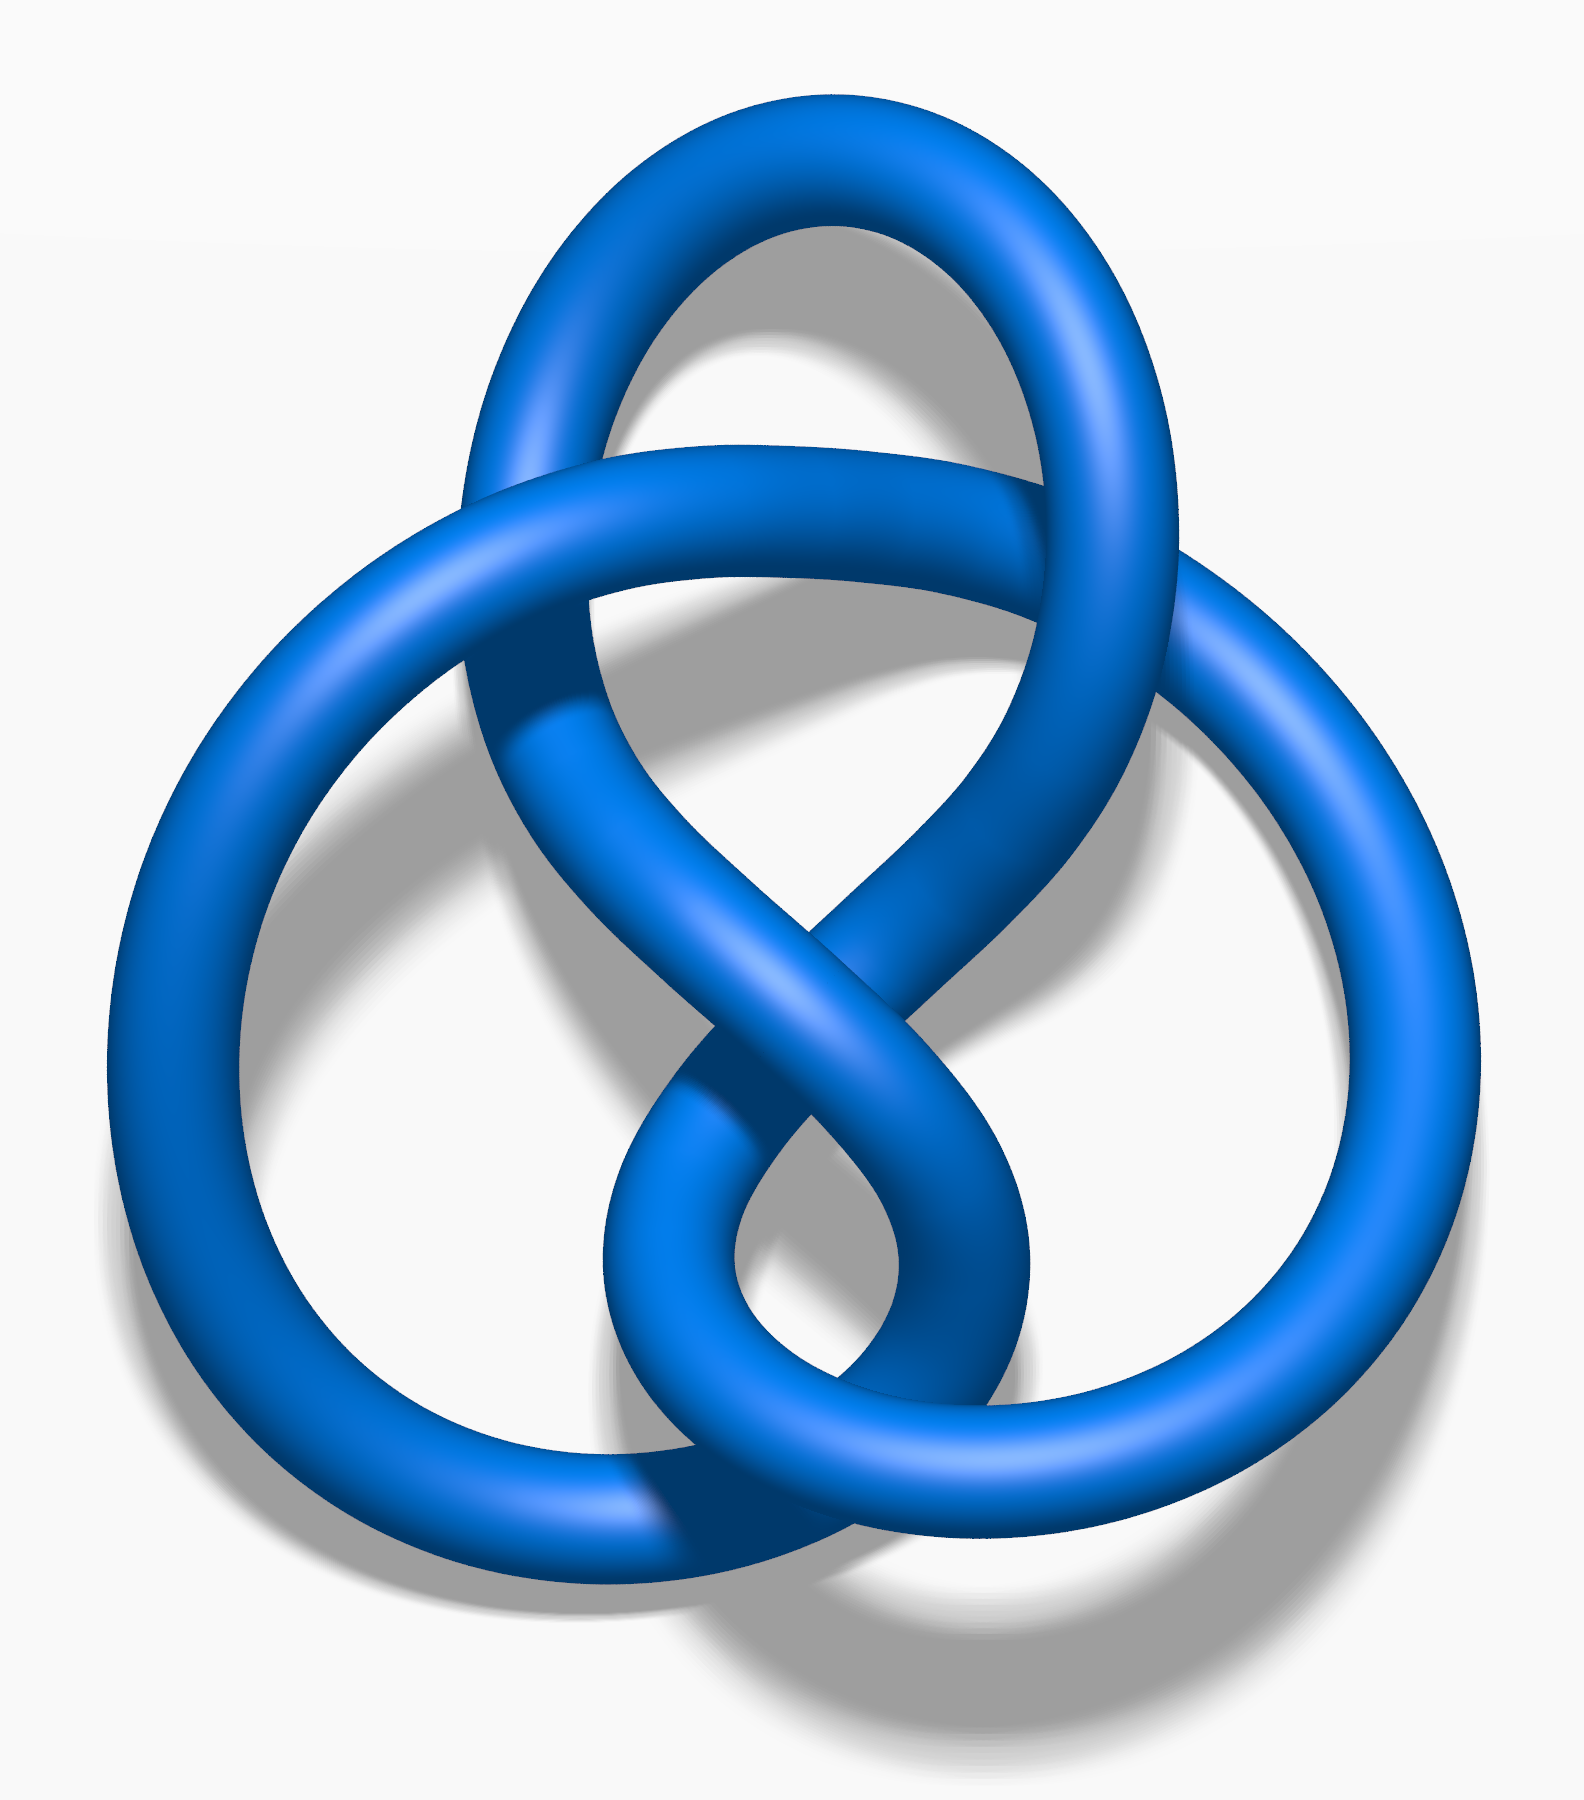
\includegraphics[width=30mm]{interesante.png}}
\caption{Una cosa interesante visual.}
\label{interesante}
\end{figure}


28:68. The Lord shall bring thee again with ships into Egypt, by the
way whereof he said to thee that thou shouldst see it no more. There
shalt thou be set to sale to thy enemies for bondmen and bondwomen, and
no man shall buy you.

28:59. The Lord shall increase thy plagues, and the plagues of thy
seed, plagues great and lasting, infirmities grievous and perpetual.

28:68. The Lord shall bring thee again with ships into Egypt, by the
way whereof he said to thee that thou shouldst see it no more. There
shalt thou be set to sale to thy enemies for bondmen and bondwomen, and
no man shall buy you.


\chapter{Conclusiones}

\section{Contribuciones}

\section{Trabajo a futuro}



\bibliographystyle{plainnat}
\bibliography{tesis}

\end{document}
